%%%%%%%%%%%%%%%%%%%%%%%%%%%%%%%%%%%%%%%%%%%%%%%%%%%%%%%%%%%%%%%%%%%%%%%%%%%%%%%%
%2345678901234567890123456789012345678901234567890123456789012345678901234567890
%        1         2         3         4         5         6         7         8

\documentclass[letterpaper, 10 pt, conference]{ieeeconf}  % Comment this line out if you need a4paper

%\documentclass[a4paper, 10pt, conference]{ieeeconf}      % Use this line for a4 paper

\IEEEoverridecommandlockouts                              % This command is only needed if 
                                                          % you want to use the \thanks command

\overrideIEEEmargins                                      % Needed to meet printer requirements.

% See the \addtolength command later in the file to balance the column lengths
% on the last page of the document

% The following packages can be found on http:\\www.ctan.org
\usepackage{graphicx} % for pdf, bitmapped graphics files
%\usepackage{epsfig} % for postscript graphics files
%\usepackage{mathptmx} % assumes new font selection scheme installed
%\usepackage{times} % assumes new font selection scheme installed
\usepackage{amsmath} % assumes amsmath package installed
\usepackage{amssymb}  % assumes amsmath package installed
\usepackage{multicol}

\title{\LARGE \bf
Hardware Trojan Implemented on a FPGA  
}


\author{Justin Cox and Tyler Travis
\\ \small{Department of Electrical and Computer Engineering}
\\ \small{Utah State University}
\\ \small{Logan, Utah 84322}
\\ \small{email: justin.n.cox@gmail.com, tyler.travis@aggiemail.usu.edu}
}

\usepackage{listings}
\usepackage{color}

\definecolor{dkgreen}{rgb}{0,0.6,0}
\definecolor{gray}{rgb}{0.5,0.5,0.5}
\definecolor{mauve}{rgb}{0.58,0,0.82}

\lstset{frame=none,
  language=C,
  aboveskip=3mm,
  belowskip=3mm,
  showstringspaces=false,
  columns=flexible,
  basicstyle={\small\ttfamily},
  numbers=none,
  numberstyle=\tiny\color{gray},
  keywordstyle=\color{blue},
  commentstyle=\color{dkgreen},
  stringstyle=\color{mauve},
  breaklines=true,
  breakatwhitespace=true,
  tabsize=3
}

\begin{document}



\maketitle
\thispagestyle{empty}
\pagestyle{empty}


%%%%%%%%%%%%%%%%%%%%%%%%%%%%%%%%%%%%%%%%%%%%%%%%%%%%%%%%%%%%%%%%%%%%%%%%%%%%%%%%
\begin{abstract}

Hardware trojans are becoming more of a threat to devices and systems as the number of ICs and chips are being manufactured and fabricated overseas.  These overseas facilities often also work with other third party company and it becomes more complex to track down where each step of the design phase takes place.  If an attacker was able to gain control of a step in the design phase, a hardware trojan could be inserted to corrupt functionality and reliability, or leak important or secret information.  This paper discusses the method of designing a hardware trojan for an FPGA.  The most effective method of defending against these hardware trojans is understanding how they are implemented.

\emph{Index Terms}---hardware trojan, data leaking, security, FPGA.

\end{abstract}

%%%%%%%%%%%%%%%%%%%%%%%%%%%%%%%%%%%%%%%%%%%%%%%%%%%%%%%%%%%%%%%%%%%%%%%%%%%%%%%%
\section{INTRODUCTION}

Hardware trojans are a great way for an attacker to leak important information such as encryption/decryption keys because, if well implemented, are hard to detect.  Since most of the ICs and chips made today are important from overseas, detected these hardware trojans is critical.  There are a few methods of detecting hardware trojans [1] which include power analysis or side-channel analysis.  This paper will discuss the implementation of a hardware trojan on an FPGA which has been synthesized to run a 8051 Intel Microprocessor architecture.  This processor has been programmed to function as a dedicated DES crypto device.   

\subsection{Previous Work}

There is current and previous research on the implementation of hardware trojans and how they are used to leak information [2].  There are even competitions designed to allow competitors to design a hardware trojan on a microprocessor.  This paper will focus on a FPGA hardware trojan implementation to leak the secret key used in the DES algorithm.  This paper will try to design a trojan with a small profile, low power requirements, and the ability to remain hidden from detection. 

%%%%%%%%%%%%%%%%%%%%%%%%%%%%%%%%%%%%%%%%%%%%%%%%%%%%%%%%%%%%%%%%%%%%%%%%%%%%%%%%

\section{8051 IP CORE}

The Intel 8051 architecture was developed by Intel in the 1980s.  Intel has allowed other companies to design their own versions of the 8051 architecture, and as a result, can be found in many embedded system designs.  Since the 8051 microcontroller is an older design, it is limited to 8-bit instructions and has a limited amount of peripherals.  This is illustrated in Figure 1 and needs to be taken into consideration when designing the hardware trojan.  

\begin{figure}[thpb]
	\centering
	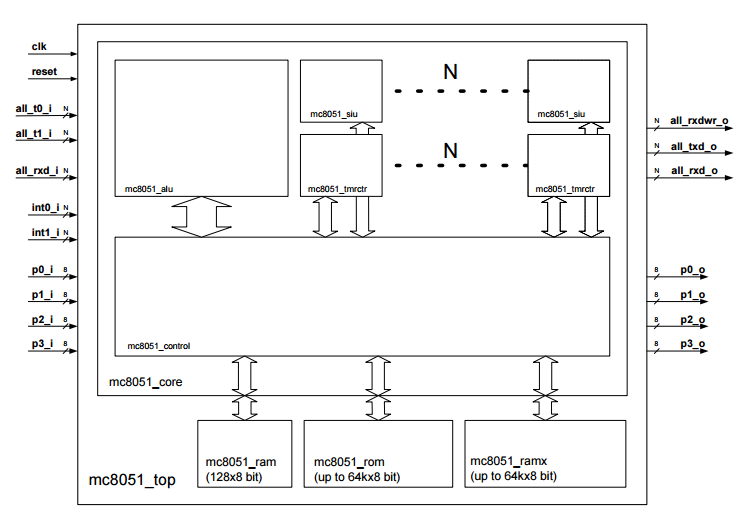
\includegraphics[scale=.50]{8051}
   \caption{System overview of the Intel 8051.}
\end{figure}

There are free 8051 IP cores available on the internet and the authors chose to use the 8051 VHDL implementation from Oregano Systems [3].  The IP core is able to have three memory modules loaded onto the FPGA design.  The 8051 is limited to 128 bits of internal RAM but the ROM and extra RAM can be designed up to 64kB of data.

Once the 8051 IP core has been loaded on the FPGA, a DES program in C needs to be loaded in order to allow encryption and decryption.

\section{TROJAN DESIGN}

There are many different ways to characterize a trojan and this paper will use the taxonomy described in the following subsection.

\subsection{Taxonomy}

Hardware trojans will be characterized based on the following metrics:

\begin{itemize}
\item Insertion
\item Abstraction
\item Activation
\item Effects
\item Location
\end{itemize}

The proposed hardware trojan, once triggered, will delay the communication lines of the UART module to leak the secret key used for encryption and decryption.  Tampering with the baudrate would likely create errors in the communication.  This trojan will maintain the designed baudrate while created different delays after each 8-bit data frame.

The trojan is inserted at the Design and Fabrication stage.  It is assumed that the attacker would have access to the netlists and hardware description code to make the necessary changes.  The trojan would be extracted at the RT level and gate level because the trojan effects the control logic as well as some gate signals.  The trojan will be activated externally by a user which decreased the chance of being detected.  The trojan will be triggered when a predetermined 6 byte chunk of the plaintext is entered into the crypto system.  The trojan design is shown further in Figure 2.

\begin{figure}[thpb]
	\centering
	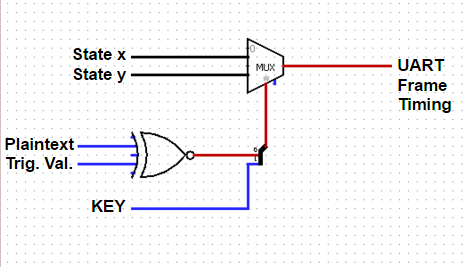
\includegraphics[scale=.50]{trojan}
   \caption{Logic design of the hardware trojan}
\end{figure}

As mentioned previously, the effect of the trojan will be the leakage of secret information.  The trojan will be located on parts of the processor and well as some of the I/O such as the RS-232 signals.

\subsection{Serial Communication}

A separate program was written in C to allow an interface for the user to input a desired plaintext to be encrypted.  The resulting cyphertext is sent over UART to the user.  The trojan is triggered when the plaintext of "0x70776e616765...” in hexadecimal or “pwnage” in ASCII is received.  The user interface of the crypto system is shown in Figure 3.

\begin{figure}[thpb]
	\centering
	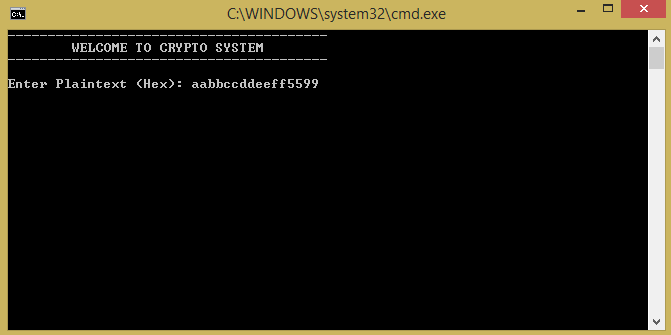
\includegraphics[scale=.50]{SerialProg}
   \caption{The UI that allows the trigger to be sent.}
\end{figure}

\subsection{Trojan Implementation}

Once the trojan is triggered, the current key bit is sent to the UART module. Once the key bit is there it will either set the TX frame to have 1 stop bit if the key bit value is a 0 or to have 2 stop bits if the key bit value is a 1. Technically 8 bits are sent per ciphertext output, but the last frame is cut off so realistically, there are only 7 bits of data per ciphertext.

  
\section{EXPERIMENTAL RESULTS}

The trojan worked as expected once everything was loaded onto the board. The spacing between the frames from the varying stop bits caused the bits for the key to be leaked out over 8 plain text inputs, with the first one being the triggering plaintext of "pwnage" or 0x7077.6e61.6765 in hex. The only part left to the person leaking the key is to brute force the remaining 8 bits left off by completed ciphertext outputs on the TX line of the FPGA.

Since the authors were not able to get the 8051 IP core completely working on the Spartan 3E FPGA, the trojan and DES system were implemented directly on the FPGA.  The UART IP Core was obtained from www.fpga4fun.com and the DES IP Core was obtained from OpenCores.  The credit of these cores are found in the source code.

\subsection{Size}
 
The size of this trogan compared others is realitiviy small compared to the other trojans in the class. With only a 6.2\% increase in look up tables (LUTs) at the worst, there isn't a lot of extra area used. Refer to Table xx for more information.

 \begin{center}
    \begin{tabular}{| l | l | l | l | l |}
        \hline
        & Original & With Trojan & Difference & Percentage \\ \hline
        LUTs & 835 & 887 & 52 & 6.2\% \\ \hline
        Slices & 562 & 587 & 25 & 4.4\% \\ \hline
        Flip Flops & 451 & 467 & 16 & 3.5\% \\
        \hline
    \end{tabular}
\end{center}

\subsection{Power}

The power that was consumed by the trojan was a little bit more than other trojans in the class. This is probably due to the size of some of the components in the design. The power was measured using a shunt resistor in series with the ground pin of the FPGA by measuring the voltage drop over the resistor to find the current through it. The power can be found by taking the supply voltage and multiplying it by the current over the resistor.

 \begin{center}
    \begin{tabular}{| l | l | l | l | l |}
        \hline
        & Original & With Trojan & Difference & Percentage \\ \hline
        Volts (supply) & 5.5 & 5.5 & 0 & 0\% \\ \hline
        Amps (supply) & 0.067 & 0.067 & 0 & 0\% \\ \hline
        Volts (resistor) & 1.72mV & 1.84mV & 0.12mV & 6.9\% \\
        Watts & 7.8mw & 8.4mW & 0.6mW & 7.69\% \\
        \hline
    \end{tabular}
\end{center}

\subsection{Detectability}

The detectability of the trojan is pretty low since the trojan is only activated when a certain event triggers it. Therefore, the output of the device will stay consistent as long as the plaintext trigger isn't entered into the device. Once the trigger has been triggered, the device will leak the key through the next 8 UART frames for the attacker to use.

\subsection{Measurements} 

Eight measurements were taken from the TX pin from the FPGA. These 8 measurements show that key is leaked through the stop bit(s) of the UART frames. 

The figures for the measurements are included in the appendix of this report.

\section{CONCLUSION}

The trojan was successfully implemented on a Spartan 3E FPGA.  The trojan does not take up a lot of extra space and would be hard to detect when analyzing the floor plan.  The trojan also was able to maintain a low power profile.  The key can be reliably extracted from the UART Tx communication line and it would only be detected if the signal was analyzed with an oscilloscope after activation.  The probably of accidentally activating the trojan is low which would also hinder the ability to test and detect the trojan.

The authors were not able to get the 8051 IP core working with a large DES code written in C.  The authors were able to learn a lot about microcontroller implementations on FPGAs and the time spent debugging the 8051 IP core was worth while. 

\addtolength{\textheight}{-12cm}   % This command serves to balance the column lengths
                                  % on the last page of the document manually. It shortens
                                  % the textheight of the last page by a suitable amount.
                                  % This command does not take effect until the next page
                                  % so it should come on the page before the last. Make
                                  % sure that you do not shorten the textheight too much.

%%%%%%%%%%%%%%%%%%%%%%%%%%%%%%%%%%%%%%%%%%%%%%%%%%%%%%%%%%%%%%%%%%%%%%%%%%%%%%%%



%%%%%%%%%%%%%%%%%%%%%%%%%%%%%%%%%%%%%%%%%%%%%%%%%%%%%%%%%%%%%%%%%%%%%%%%%%%%%%%%



%%%%%%%%%%%%%%%%%%%%%%%%%%%%%%%%%%%%%%%%%%%%%%%%%%%%%%%%%%%%%%%%%%%%%%%%%%%%%%%%

%\section*{ACKNOWLEDGMENT}

%The author would like to thank his instructor Dr. Rajnikant Sharma %for his help in understanding control concepts.




%%%%%%%%%%%%%%%%%%%%%%%%%%%%%%%%%%%%%%%%%%%%%%%%%%%%%%%%%%%%%%%%%%%%%%%%%%%%%%%%


\begin{thebibliography}{99}

\bibitem{c1} M. Ganga and M. Hsiao, "A Novel Sustained Vector Technique for the Detection of Hardware Trojans", International Conference on VLSI Desgin, 2009.
\bibitem{c2} A. Baumgarten, M. Clausman, B. Lindenmann, M. Steffen, B. Trotter and J. Zambreno, "Embedded Systems Challenge", 2008.
\bibitem{c3} "8051 IP Core » Oregano Systems", Oreganosystems.at, 2016. [Online]. Available: http://www.oreganosystems.at/?page\_id=96. [Accessed: 06- May- 2016].

\end{thebibliography}

\end{document}
